\chapter{Estudio de Reuseport}

Como ya se estudió, los problemas del escenario multithreading reconocidos en el capítulo anterior impactan principalmente en los tiempos de operaciones de tareas en que el tráfico y, por ende, el tiempo de respuesta, es un elemento prioritario a garantizar. Entendiendo éste problema es que varios gigantes de la industria han planteado mecanismos alternativos que permitan aprovechar mejor los recursos de los computadores de arquitecturas modernas al emplear programación paralela ???????????. En ésta linea, la propuesta más prometedora hasta la fecha es la brindada por Google, denominada \emph{Reuseport}.

\emph{Reuseport} \cite{slides:googleReuseport} es una de las soluciones más usadas para el problema descrito por su gran efectividad en la practica. Corresponde a un desarrollo de Tom Herbert --Ingeniero de Google-- desarrollado precisamente para atender los bajos desempeños generados a emplear un esquema de consumo de sockets como el planteado hasta el momento. El trabajo de Herbert plantea que las distintas estratégias que se puedan adoptar sobre un único socket para mejorar la performance en su acceso concurrente terminan no resultando efectivas por mantener el punto de contención al compartir la misma estructura.

\begin{figure}[h!]
	\centering
	\hspace*{\fill}
	\subfigure[Socket Tradicional]{
		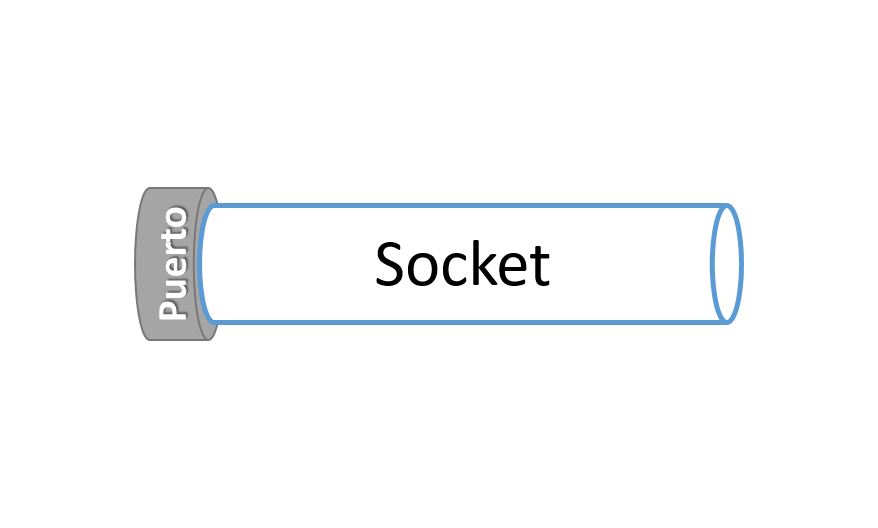
\includegraphics[width=.45\textwidth]{imagenes/socketNormal.png}
	}\hfill
	\subfigure[Socket con opción Reuseport activada]{
		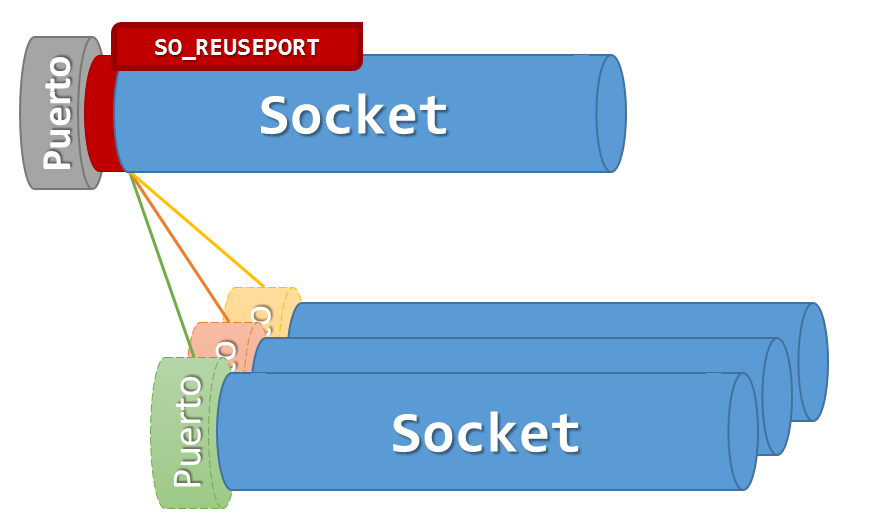
\includegraphics[width=.45\textwidth]{imagenes/socketReuseport.png}
		\label{fig:soReuseport}
	}
	\caption{Comparativo del funcionamiento de sockets tradicionales con respecto a Reuseport. En éste último, basta con que el primer socket que enlace al puerto en cuestión tenga la opción habilitada para que cualquier socket posterior se pueda sobre acomplar sobre el mismo puerto, compartiendo así el consumo de datos del mismo.}
	\label{fig:socketHandshake}
	\hspace*{\fill}
\end{figure}

Reuseport se plantea como una opción para los sockets estándar de Linux que promete una mejora en los tiempos de consumo en la atención a un determinado puerto. Dicha opción permite compartir un mismo puerto local del sistema entre múltiples sockets distintos. De ésta manera, conservando el esquema multithread, cada thread puede tener exclusividad en el consumo de un socket, eliminando el punto de contención único que se ocaciona al compartir un sólo socket. Al usar la opción \emph{Reuseport}, la tarea de distribución de paquetes entre los distintos sockets que compartan un puerto local es delegada directamente al kernel, el cual asigna aleatoreamente los paquetes recibidos entre los sockets que escuchan el mismo puerto.

\section{Implementación}
La opción está implementada íntegramente en el código fuente del kernel, distribuida entre distintos archivos que hacen uso de la misma. Por sólo mencionar algunos, los archivos 


\section{Uso en la práctica}
La adopción de ésta funcionalidad ha sido incorporada a software con requerimientos de alta disponibilidad de atención de consultas con buenos resultados \cite{paper:apache}. En la práctica, para usar ésta opción se debe modificar la estructura socket que primero tome control del puerto local para escucharlo por medio de la llamada \verb=bind()=. Ello se puede hacer por medio de la llamada de sistema \verb=setsockopt()= con la cual se puede modificar el descriptor de una estrutura socket. En éste punto es necesario entregar la constante \verb=SO_REUSEPORT= como una opción para activar en la estructura socket. Con ello, el puerto puede ser posteriormente re-acoplado por otros sockets sin la necesidad de que éstos últimos tengan la característica activada (Ver imagen \ref{fig:soReuseport}).

\section{Rendimiento}
Para evaluar el rendimiento práctico de la opción \emph{reuseport} se modificó sutilmente el caso de estudio evaluado a lo largo de la investigación apra hacerlo compatible para con éste enfoque de solución. Al igual que en el escenario original, el objetivo es calcular el tiempo de consumo de 1G de paquetes desde un socket UDP en escenario de saturación. La diferencia en éste caso radica en que, en pos de aprovechar las promesas de \emph{reuseport}, se cambia el consumo concurrente desde el mismo socket usando múltiples hilos por un consumo de múltiple hilos que consume cada uno a un socket distinto, alocado en la misma interzaf lógica del sistema del socket saturado. De ésta manera, el consumo por socket ahora es exclusivo para cada thread y eliminando ese punto de contención de la prueba original.

\begin{figure}[!h]
	\centering
	
\includegraphics[scale=.3]{imagenes/fcfm}
	\caption{Nuevo esquema de la prueba UDP en escenarios donde se aproveche Reuseport.}
	\label{fig:casoPruebaReuseport}
\end{figure}

Así mismo, se definen los siguientes conceptos a tener presentes en este nuevo caso de estudio:
\begin{description}
\item[Tiempo Mínimo] Corresponde al tiempo en que el primer socket termina de consumir su cuota asignada.
\item[Tiempo Neto] Corresponde al tiempo en que el último socket termina de consumir su cuota asignada. De esta forma, corresponde al tiempo en que se completa la trasferencia total.
\item[Cuota de Consumo] Corresponde a la porción de paquetes que le corresponde consumir a cada socket. Si el envío total se denomina como $N$ y se tienen $k$ sockets para emplear el consumo con reuseport, la cuota de consumo de cada uno es el cociente $\frac{N}{k}$.
\end{description}

Para poder llevar a cabo ésta prueba, es necesario garantizar que el primer socket creado para la recepción de información posea la opción \verb=SO_REUSEPORT= habilitada, además la cantidad total de consumo (1G de paquetes) debe ser redistribuida entre los sockets que se evalúen, asignando una \textbf{cuota de consumo} a cada socket de lectura que en conjunto sume la cantidad neta del caso de prueba original. La medición de tiempos en éste caso debe ser en función del último socket que termine el consumo de su cuota, pues dicho tiempo representa el tiempo total en que se completa la transferencia total en relación al caso de estudio original. Un esquemático de ésta prueba puede apreciarse en la figura \ref{fig:casoPruebaReuseport}.

\subsection{Diferencias entre arquitecturas}


\section{Evaluación de Optimizaciones Adicionales}
Los resultados anteriores evidencian un claro incremento en el rendimiento alcanzable por la prueba ya conocida aprovechando múltiples hilos de ejecución. Sin embargo cabe preguntarse si será posible mejorar aún más esos resultados combinando la opción de \emph{Reuseport} con técnicas de consumo concurrente sobre los sockets. Una hipótesis que apoya ésta idea se basa en que, al emplear la opción \emph{Reuseport} los sockets tienen una menor cuota de consumo cada uno, por lo tanto, un acceso concurrente en ese escenario de bajo consumo podría impactar en una reducción de tiempos finales.

En la presente sección se validará el rendimiento alcanzable por la opción \emph{Reuseport} usándola en combinación con diferentes estratégias de multithreading como las vistas en el capítulo anterior.

\subsection{Incorporación de Multithreading}

\subsection{Incorporación de Multithreading con Processor Affinity}
Similar al estudio del capítulo anterior en la arista de distribución de carga, se evaluó el desempeño de Reuseport en escenarios donde múltiples hilos de consumo al socket fuesen distribuido lógicamente entre los distintos CPU del sistema aprovechando la técnica de \emph{Processor Affinity}. En éste caso, se evaluaron 3 configuraciones:

\begin{description}
\item[All0] Los distintos hilos de ejecución se alocan en el mismo core (core 0 por simplicidad). Persigue aprovechar localidad de datos en la ejecución simultanea de los hilos.
\item[Equitative] Los hilos se distribuyen equitativamente entre los cores lógicos del sistema, persiguiendo una distribución de carga entre unidades de procesamiento real.
\item[SO] Los hilos son distribuidos por el mismo sistema operativo a través de la oepración de su algoritmo de \emph{schedulling}. Es la base de comparación para con los demás esquemas de distribución.
\end{description}

\subsection{Análisis y Discusión de Resultados}
Como se aprecia de los resultados experimentales, la incorporación de multithreading en el consumo de datos desde una estructura socket con soporte para \emph{reuseport} siempre degrada el rendimiento completo del caso de estudio, independiente de si se emplean esquemas de distribución de carga entre los núcleos de procesamiento efectivo. Resulta interesante que más allá de las estratégias que se adopten para la mejor distribución de carga, las variaciones no permiten justificar una verdadera ganancia o pérdida entre esquemas que se adopten, siendo simplemente sobrecargas con respecto al esquema de distribución propio del sistema oeprativo.

Éste resultado viene a confirmar la conclusión de los estudios del capítulo anterior que terminan por postular que es la misma estructura socket de Linux la que no cuenta con un diseño compatible con técnicas de consumo concurrente, degenerando siempre en escenarios de degradación de performance generalizada en su consumo.

\section{Aspectos Negativos}

El esquema que propone Reuseport re-plantea uno de los principios fundamentales que postula el modelo OSI, que es la relación uno a uno entre estructuras sockets y direcciones de puertos locales. Como \emph{Reuseport} plantea la copartición de puertos locales, se pierde la exclusividad de los mismos para cada socket. Otra caracteristica que trastoca ésta alternativa es la modificación en la manera de programación de aplicaciones. Como se mencionó, el uso de \emph{Reuseport} está condicionado a la habilitación de dicha opción a los sockets previo al momento de su acoplamiento con el puerto local a escuchar. Ésta situación significa en la práctica estar concientes de que toda aplicación que desee hacer uso de ésta característica debe modificar secciones profundas de su impleentación en el código fuente para habilitarla.

Por otro lado, dado su funcionamiento la opción de \emph{Reuseport} está incorporada como código fuente del kernel de Linux, estando disponible según sus creadores en los kernels con versiones posteriores a la 3.9 (Finales del año 2013), ello no es del todo correcto. Conocido es el caso de las distribuciones de Linux basadas en Debian --incluido el popular Ubuntu-- donde se han presentado varios problemas en versiones recientes las cuales, a pesar de contar con la implementación fuente de \emph{Reuseport}, poseen la constante de activación de la característica como código comentado [AKA UNA REF. A ALGO QUE JUSTIFIQUE ESTO], lo cual dificulta el uso de ésta opción al no dejarla disponible para el uso de los programadores de aplicaciones o llevando a errores de programas en el peor caso.

Una última dificultad asociada al uso de la opción \emph{Reuseport} se relaciona con su documentación. La documentación asociada a ésta característica es muy escasa, reducíendose prácticamente a la implementación misma, disponible en el código fuente del propio kernel de Linux. No existe documentación a nivel de usuario que permita comprender ni mucho menos manipular las características de la opción en sí misma. En esa misma linea, aparece como un problema la implementación de ésta característica. Al ser una opción \emph{Hardcodeada} en el kernel mismo de Linux resulta inviable pensar cualquier modificación doméstica pensando en querer aprovechar de su funcionamiento con ciertas modificaciones, ello pues significaría modificar, recompilar e instalar todo el nuevo kernel, manteniendo el riesgo de posibles inestabilidades del resultado, algo que en la práctica es dificilmente aceptable. Ésto último da a entender que la característica \emph{Reuseport} no está pensada para ser modificable según escenarios especificos de operación.